% \errorstopmode %  stop on error
\batchmode %  disable output generation
% preambolo per doppia compilazione HTML/PDF
\ifx\pdfoutput\undefined      % compilazione htlatex
\documentclass{article}
\DeclareGraphicsExtensions{.png, .gif, .jpg}

\else                         % compilazione pdflatex
\documentclass{article}

% packages
\usepackage{graphicx}
\usepackage{listings}
\usepackage{fancyhdr}
\usepackage{wrapfig}
\usepackage{multirow}
\usepackage{lscape}
\usepackage{amssymb,amsmath}
\usepackage[hyperindex]{hyperref}

% page setup
\pdfpagewidth 8.5in
\pdfpageheight 11in
\setlength\textwidth{5.7in}
\setlength\textheight{8.1in}
\setlength\oddsidemargin{0in}
\setlength\evensidemargin{0in}
\setlength\topmargin{-0.6in}
\setlength\footskip{0.6in}
\setlength\headsep{0.6in}

% custom commands
\newcommand{\percent}{\,^0\!/_0}

%\newcommand{\href}[2]{\Link[#1]{}{} #2 \EndLink}
%\renewcommand{\hypertarget}[2]{\Link[]{}{#1} #2 \EndLink}
%\renewcommand{\hyperlink}[2]{\Link[]{#1}{} #2 \EndLink}

\hypersetup{
    pdfnewwindow=true,      % links in new window
    colorlinks=true,        % false: boxed links; true: colored links
    linkcolor=blue,          % color of internal links
    citecolor=magenta,      % color of links to bibliography
    urlcolor=blue           % color of external links
}
\fi


\begin{document}
\pagestyle{fancy}
\renewcommand{\sectionmark}[1]{\markright{\slshape \thesection\ #1}{}}
\fancyhead[R]{\bf\rightmark} 
\fancyhead[L]{e1-6 analysis}
\fancyfoot[L]{ \sl UCONN/JLAB}

% author should reflect on the fancyfoot
\author{M. Ungaro, K. Joo}
\fancyfoot[R]{ \sl M. Ungaro, K. Joo}
\title{\large e1-6 Electron Fiducial Cuts}
\maketitle

\abstract{This document describes the identification and removal of CLAS regions
of low/zero efficiency and of border effects not reproducible by GSIM.}

\tableofcontents

\section{Fiducial Cuts}

\subsection{Introduction}

A fiducial cut on electrons is introduced to constrain regions of phase space
where the CLAS response peaks at its maximum and remains rather smooth.
Furthermore, some detector inefficiencies are not perfectly reproduced with GSIM and need to be
removed with dedicated cuts.

The fiducial regions were traditionally defined in the lab coordinates of the electron reconstructed $\phi, \theta, p$.
However, it is more natural to define the fiducial regions in the detector coordinates, because
the inefficiencies are caused by tracks near their borders or hardware problems.

Since the original approach has been used in several published CLAS papers, we will include it in this note
as a reference.

\subsection{Traditional cuts on the electron lab coordinates $\phi, \theta, p$}
The fiducial cut in the lab coordinates has been determined during the $\pi^0$ analysis in
the $\Delta(1232)$ region \cite{bib:pi0_Delta}.
For each sector, an empirical cut on $\phi$ is introduced as a function of theta and momentum:
$$
\phi \,\,\le\,\, \Delta\phi \,(\theta, p)
$$
which is aimed to define regions of phase space whose distributions are flat in $\phi$.
After careful studies, and following a common approach between different CLAS experiments, the mathematical
form of the cut depends on 6 parameters  $C_i$
and assumes the form:\vspace{-0.3 cm}
$$
\begin{array}{c c c}
    \\
    \Delta\phi   & = & C_4 \left( \sin (\theta - \theta_{cut}) \right) ^{\,E} \\
    \\
    E        & = & C_3\, p\, ^{C_5} \\
    \\
    \theta_{cut} & = & C_1 + \frac{C_2}{p + C_6}
\end{array}
$$

The $\phi$ vs $\theta$ distribution were divided in 10 different momentum bins from $1.6$ to $4.6$ GeV.
Fig.~\ref{fig:fidu_etph} shows one example ($p=1.9-2.2$ GeV) of such distributions.
The $\phi$ distributions are also plotted for $\theta$ slices one degree wide as in Fig.~\ref{fig:fidu_ephis}
and the $C_i$ parameters are adjusted empirically.

Table \ref{tab:fid_epars} shows the 6 parameters obtained. Fig.~\ref{fig:fidu_e3d} shows
the fiducial cut as a function of $p$, $\theta$ and $\phi$ for sector 1.

\begin{table}[h]
    \begin{center}
        \begin{tabular}{|c|c|c|c|c|c|c|}
            \hline
            Sector & $C_1$ & $C_2$ & $C_3$ & $C_4$ & $C_5$    & $C_6$ \\
            \hline
            1      & 12.0  & 20.0  & 0.32  & 32.0  & 0.416667 & 0.14  \\
            2      & //    & 20.7  & 0.36  & 34.0  & //       & //    \\
            3      & //    & 20.2  & 0.32  & 32.0  & //       & //    \\
            4      & //    & 20.5  & 0.32  & 32.0  & //       & //    \\
            5      & //    & 20.5  & 0.29  & 32.0  & //       & //    \\
            6      & //    & 20.0  & 0.32  & 32.0  & //       & //    \\
            \hline
        \end{tabular}
    \end{center}
    \caption[The 6 parameters for electron fiducial cut for each of the 6 sectors.]
    { The 6 parameters for electron fiducial cut for each of the 6 sectors.
    Only $C_2$, $C_3$, $C_4$ are sector dependent. }
    \label{tab:fid_epars}
\end{table}


\begin{figure}[h]
    \centering
    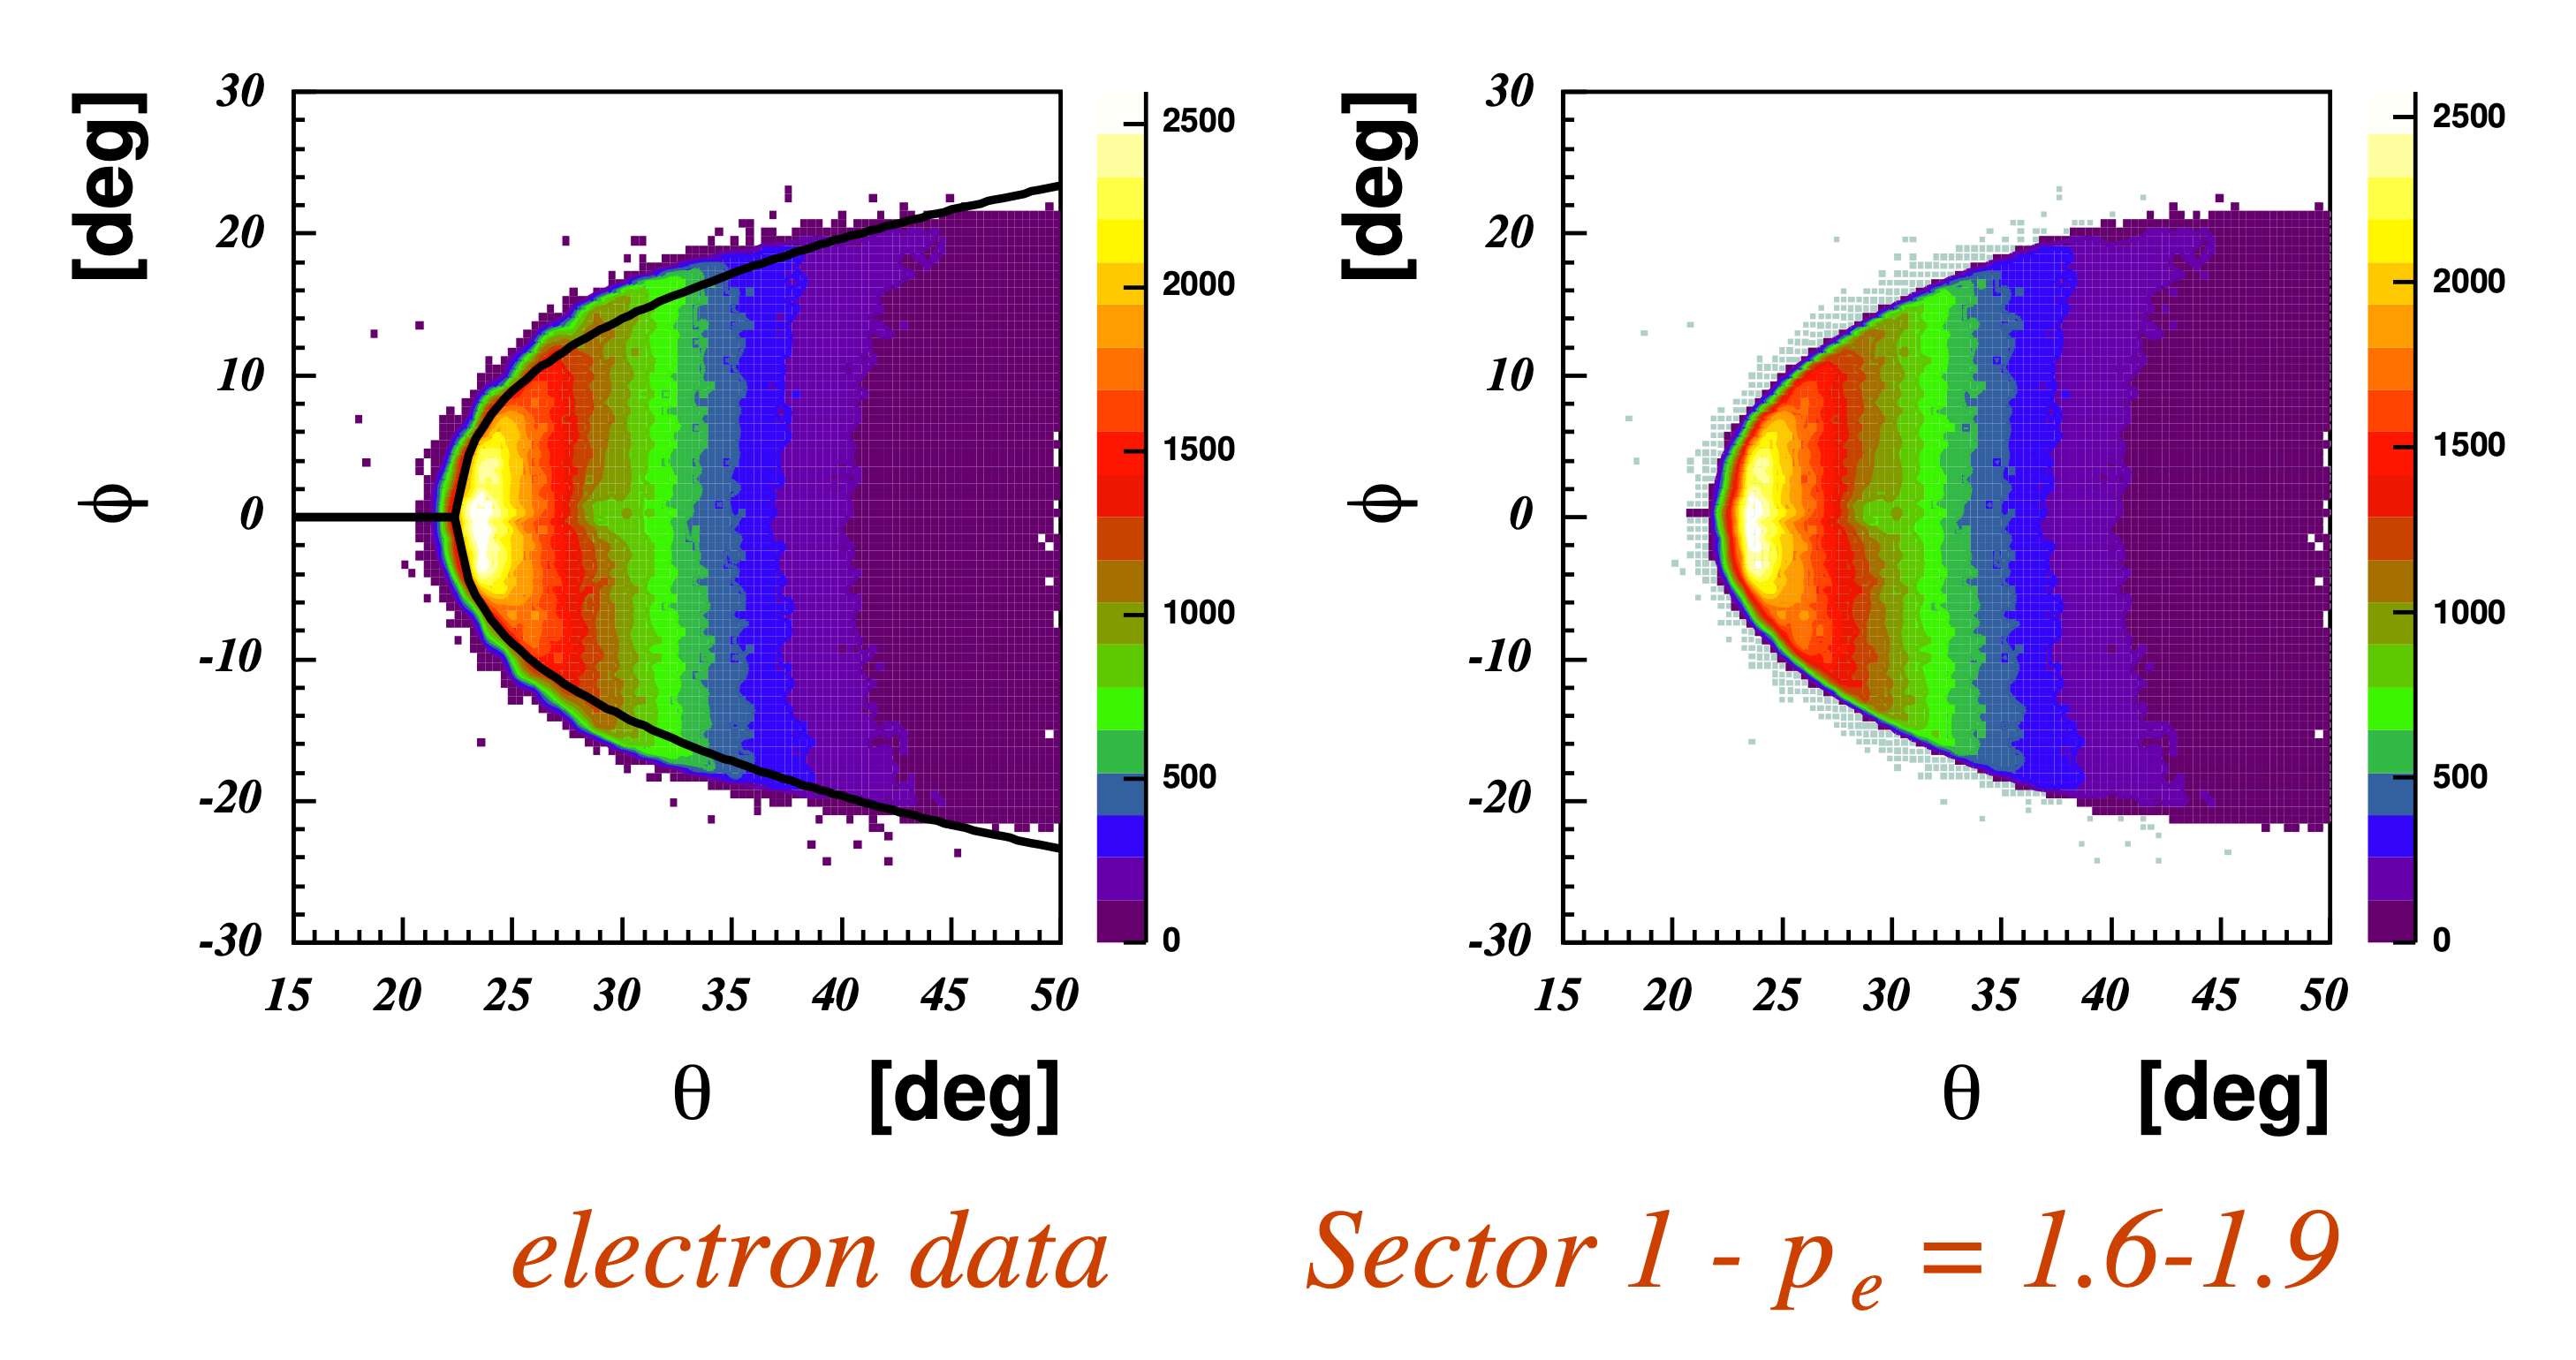
\includegraphics[width=0.9\textwidth ]{img/electron_tph}
    \caption{$\phi$ versus $\theta$ for sector 1 and $p=1.6-1.9$ GeV after the
    electron ID. Left: before fiducial cut. Right: before fiducial cut
        (box/gray) and after fiducial cut (color contour). }
    \label{fig:fidu_etph}
\end{figure}

\begin{figure}[h]
    \centering
    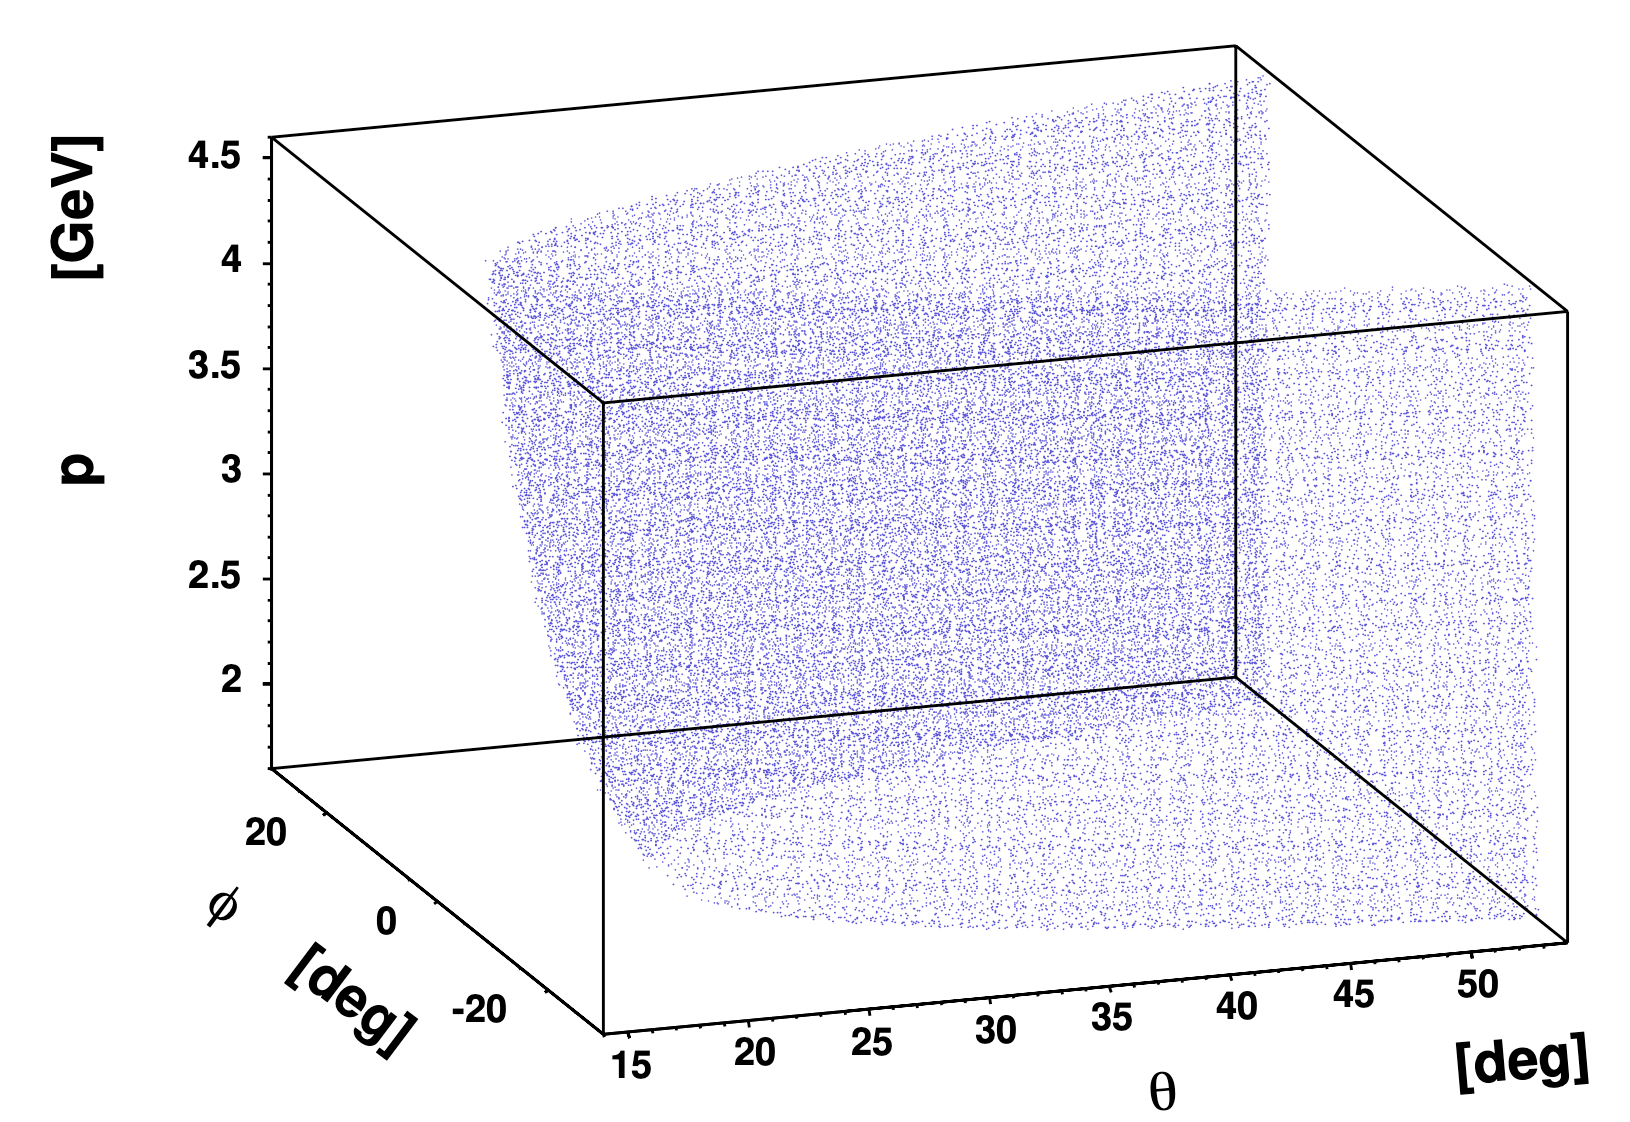
\includegraphics[width=0.9\textwidth ]{img/electron_tphp}
    \caption{The electron fiducial cut for sector 1 as a function of  $\phi, \theta, p$.
    The cut starting point moves back
    as the momentum increases (and $\theta$ decreases). This causes the cut
    to narrow up with momemtum because electrons are detected near the lower
    edges of the detectors.}
    \label{fig:fidu_e3d}
\end{figure}



\clearpage\newpage


\begin{figure}[ht]
    \centering
    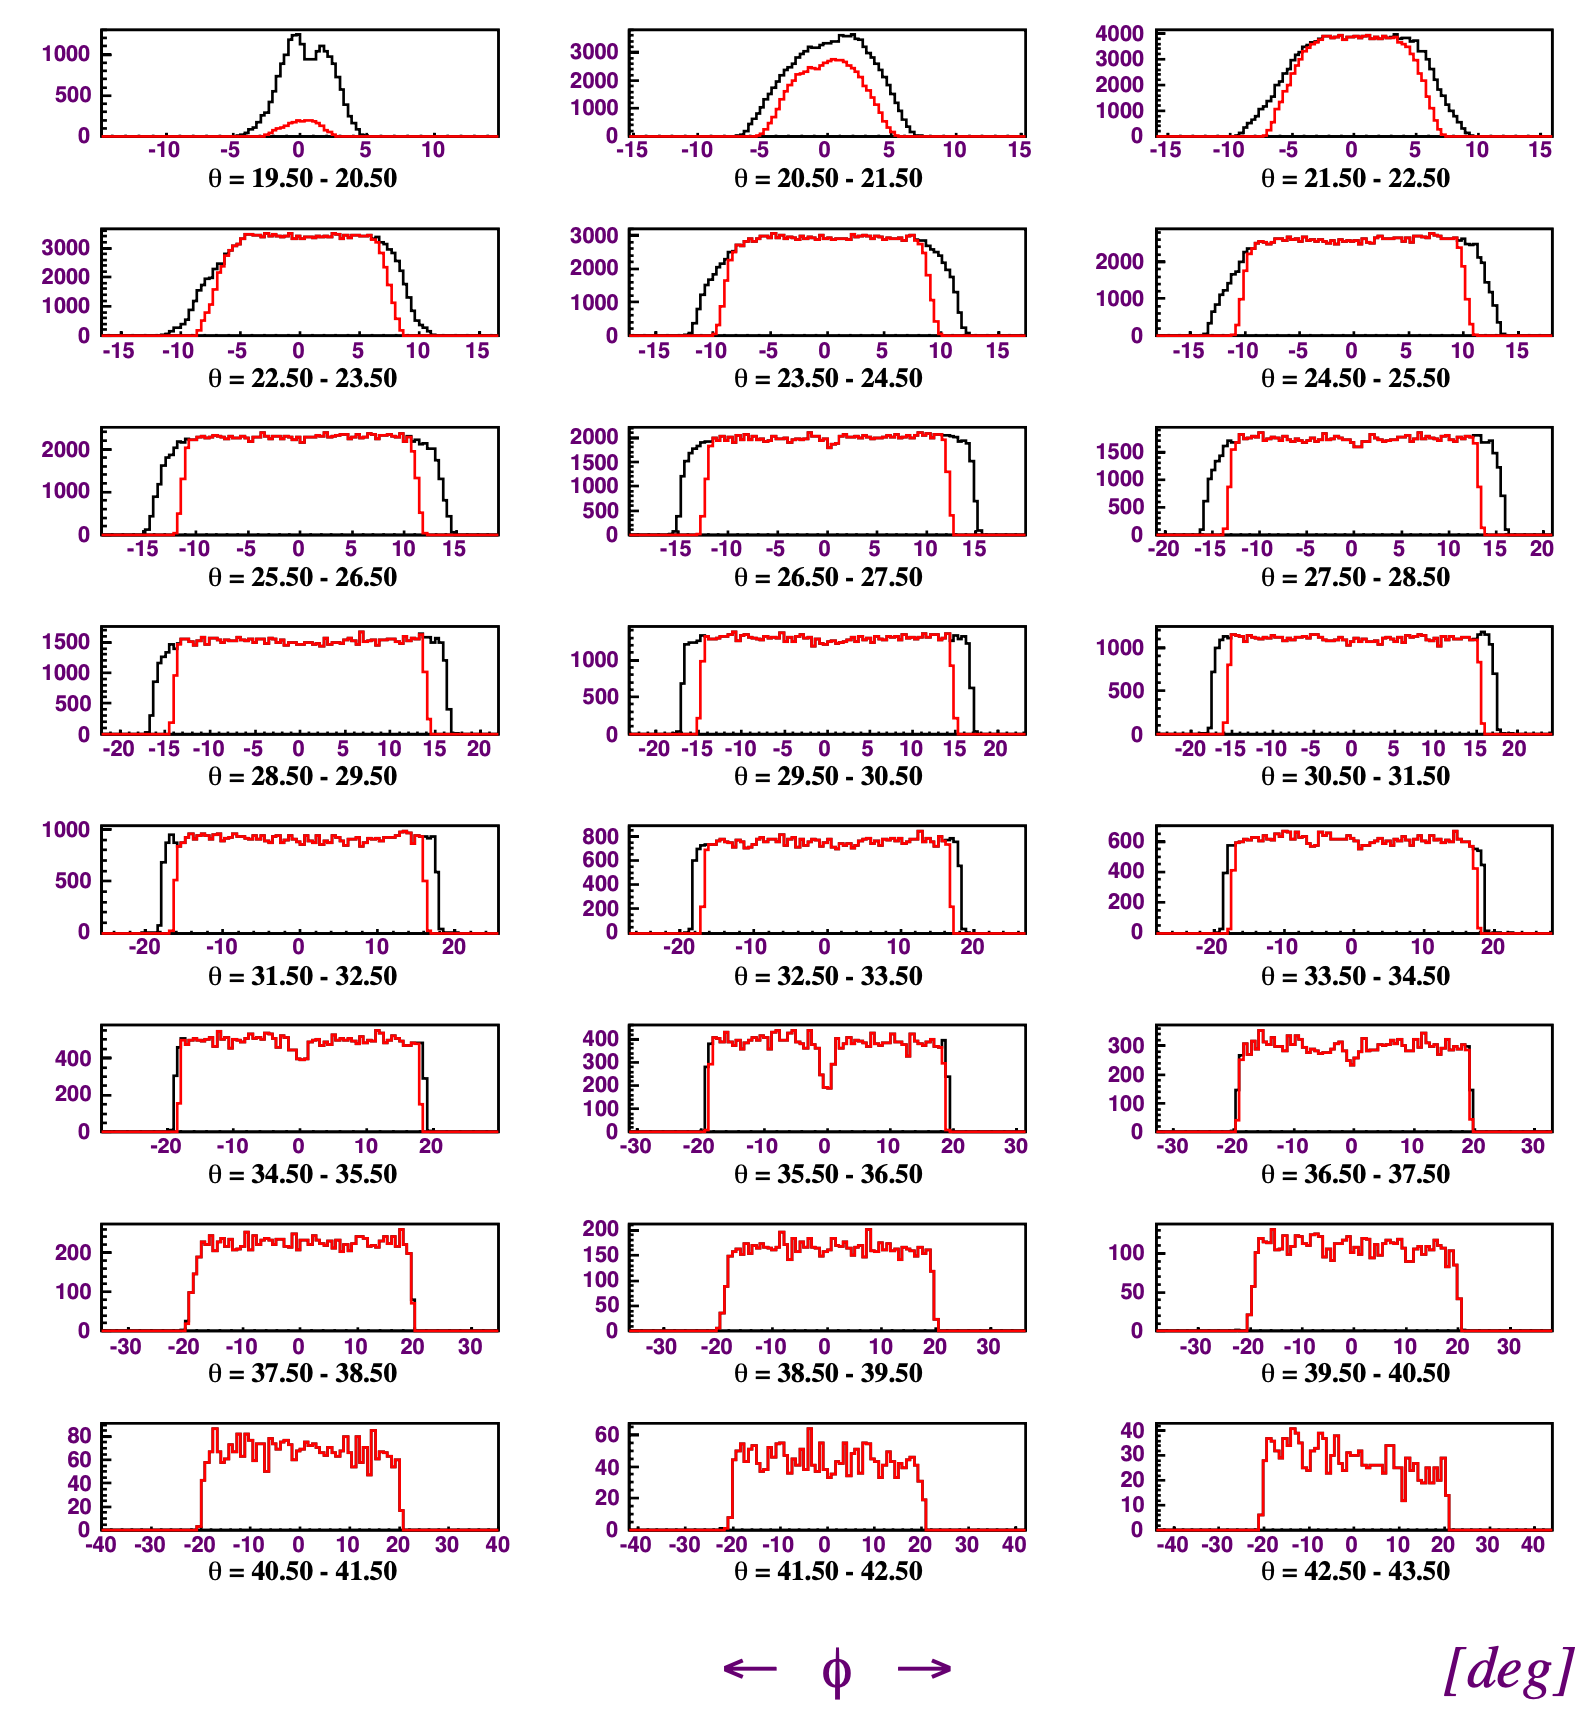
\includegraphics[width=0.98\textwidth ]{img/electron_phis}
    \caption{$\phi$ distributions (sector 3) for different $\theta$ and
        $p=1.9-2.2$ GeV. Black: before fiducial cut. Red: after fiducial cut.
        \v Cerenkov inefficiency (section \ref{sec:cc_eff}) is responsible
        for some irregularities at $\phi = 0$ (for example at
        $\theta = 35.5^0 - 36.5^0$) while drift chambers and time of flight
        inefficiency (section \ref{sec:dc_ineff}) causes other irregularities
        (for example at  $\theta = 42.5^0 - 43.5^0$).}
    \label{fig:fidu_ephis}
\end{figure}


\clearpage\newpage




\subsection{ $\theta$ versus momentum cuts}
Sector 2, 5 and 6 present holes and depletions (mainly because of dead time of flight paddles)
which were taken care of with the
cuts in the $\theta$ vs $p$ plane. An example of such cut is shown in Fig.~\ref{fig:fidu_etp5}.
The shortcomings using the electron track lab kinematics variable
is particularly evident in these  $\theta$ versus momentum cuts: there is no basis
for the functions utilised and their distances from the depletions, other than
their empirical ()visual) approximation.

\begin{figure}[h]
 \begin{center}
 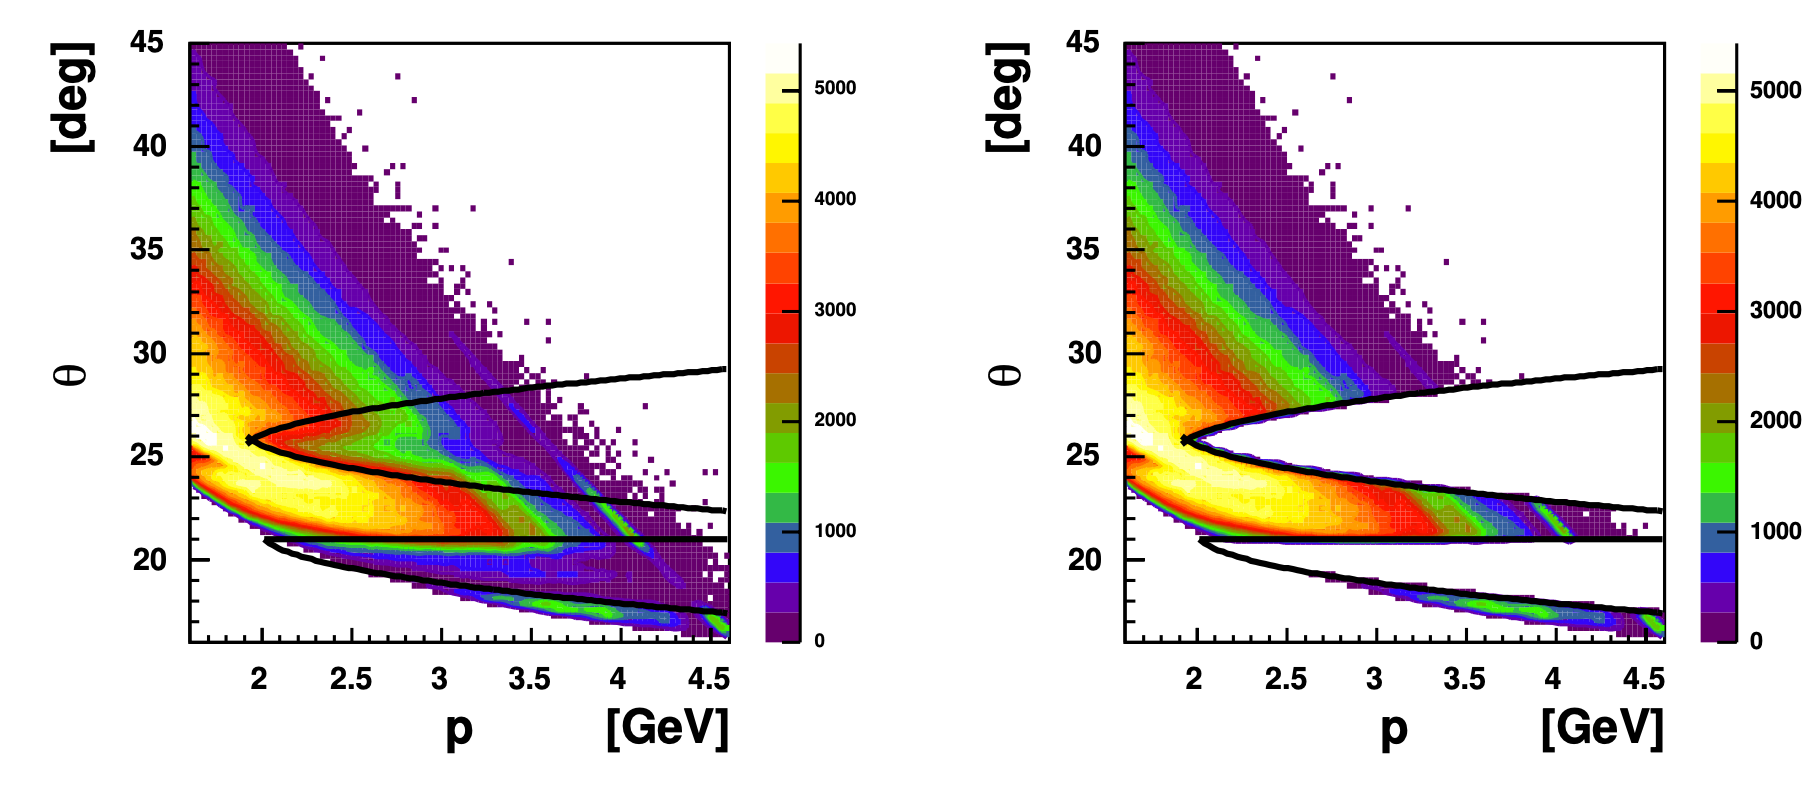
\includegraphics[width=0.98\textwidth ]{img/electron_tp5}
  \caption[ $\theta$ versus $p$ for sector 5]
          { $\theta$ versus $p$ for sector 5. Two depletions are clearly visible and cut out.}
 \label{fig:fidu_etp5}
 \end{center}
\end{figure}




\subsection{Cuts on detectors coordinates}

As the electrons swim through the detectors, they are subject to inefficiencies near the sector edges.
This applies to the 3 regions of the drift chambers (DC1, DC2, DC3) and the time of flight detector plane (SC).
An edge cut for the calorimeter was already applied in the electron ID\@.

\newpage

The X vs Y distributions of the electron tracks in the DCs and the SC planes in sector 1 are shown in Fig.~\ref{fig:xy_all_planes_s1}.
This section describes the algorithm used to select thigh occupancy regions edges.

\begin{figure}[h]
    \centering
    \includegraphics[width=0.48\textwidth ]{img/plane-DC1_intsector-1}
    \includegraphics[width=0.48\textwidth ]{img/plane-DC2_intsector-1}
    \includegraphics[width=0.48\textwidth ]{img/plane-DC3_intsector-1}
    \includegraphics[width=0.48\textwidth ]{img/plane-SC_intsector-1}
    \caption{The X vs Y distribution of the tracks in the drift chambers and the time
    of flight detector plane (SC) for sector 1. The edges selection algoritm described in the text resulted
    in the black lines, which are the fit of the Y distributions for each X bin.}
    \label{fig:xy_all_planes_s1}
\end{figure}

In each sector and each plane, 12 bins in X are defined; in each bin, the Y distribution
is fitted with a ``tent'' function $t(y)$ (defined in appendix~\ref{sec:tent_function} ) to select the high efficiency edges.
An example of such fit is show in Fig.~\ref{fig:y_slices_s1} for sector 1 in the DC3 plane, for 4 bins in X\@.
The fit cleanly identifies the steep rises and falls of the distributions and the relatively flat regions in between.

\clearpage\newpage

\begin{figure}[h]
    \centering
    \includegraphics[width=0.47\textwidth ]{img/slice-05_sector-1_plane-DC3}
    \includegraphics[width=0.47\textwidth ]{img/slice-06_sector-1_plane-DC3}
    \includegraphics[width=0.47\textwidth ]{img/slice-07_sector-1_plane-DC3}
    \includegraphics[width=0.47\textwidth ]{img/slice-08_sector-1_plane-DC3}
    \caption{Y distribution for 4 X bins in the DC3 plane for sector 1. The black lines are the
    tent fit of the Y distributions. The result of the first is the two points of intersection between the
    straight lines (steep rise) and the parabole fit (flat region). The two points are then plotted in the XY
    plane and fitted with a parabola, see for example Fig.~\ref{fig:xy_all_planes_s1} or Fig.~\ref{fig:xy_dc12_s5}.}
    \label{fig:y_slices_s1}
\end{figure}

The results of the tent fit are the two points of intersection between the straight lines (steep rise)
and the parabola fit (flat region). The two points are then plotted in the XY plane for all the X bins
and fitted with a parabola, see for example  Fig.~\ref{fig:xy_all_planes_s1} or Fig.~\ref{fig:xy_dc12_s5}.

This procedure results in a fiducial cut function for each plane and each sector.

\clearpage\newpage

\subsubsection{Detectors inefficiencies}
The detector coordinates plots allow to correlate hardware inefficiencies with depletions in the XY distributions.
For example, in the DC planes, where neighboring group of wires are powered by the same HV supply and
axial and stereo wires are tilted by $6^0$ with respect to each other, the inefficiencies
will appear as:

\begin{itemize}
    \item Axial wires: horizontal bands in the XY distributions
    \item Stereo wires: $6^0$ tilted bands in the XY distributions
\end{itemize}

Three examples of such hardware problems are summarized in Fig.~\ref{fig:xy_dc12_s5}.
These regions are removed with dedicated cuts represented by straight lines in the XY plane,
horizontal for the axial wires and $6^0$ tilted for the stereo wires.


\begin{figure}[ht]
    \centering
    \includegraphics[width=0.48\textwidth ]{img/plane-DC2_intsector-5}
    \includegraphics[width=0.48\textwidth ]{img/plane-DC1_intsector-5}
    \caption{The X vs Y distribution of the electron tracks intersection wiht the DC2 (left)
        and DC1 (right) planes in sector 5. The left distributions shows one depletion for the stereo wires,
        while the right distribution shows two depletions for the axial wires.}
    \label{fig:xy_dc12_s5}
\end{figure}

\subsubsection{Comparison with the traditional cuts}

The effect of the fiducial and inefficiencies cuts are compared with the traditional $\phi, \theta, p$ cuts.
The comparison highlights the advantages of the new approach:

\begin{itemize}
    \item identify the real edge effects in the detector
    \item hardware problems are represented by straight lines in the XY plane
    \item no momentum dependence of the cuts
\end{itemize}
This comparison is shown as an example for sector 5 and a momentum bin in Fig.~\ref{fig:PnPvsTmom-3.8_sector-5_plot-phiVsTheta}.
The before and after $\phi$ vs $\theta$ distributions in sector 5 for all the momentum bin are shown in Fig.~\ref{fig:phiTheta-before_sector-5}
and~\ref{fig:phiTheta-after_sector-5} respectively.

The complete set of plots is available at ~\cite{bib:pi0_resonance_fiducial_electron}.

\begin{figure}[ht]
    \centering
    \includegraphics[width=0.98\textwidth ]{img/PnPvsTmom-3.8_sector-5_plot-phiVsTheta}
    \caption{Comparison between the traditional cuts (function of $\phi, \theta, p$) and the new cuts on the XY detector coordinates.
    Top left:  $\phi$ vs $\theta$ before any cuts. Top right:  $\phi$ vs $\theta$ after the XY cuts cuts. The traditional cuts superimposed
    and shown with black lines. Notice that the traditional cuts would remove events at very small $\theta$ and large $\phi$, due to its functional form.
    Bottom left: DC1 plane after the fidu XY cuts. Bottm right: DC2 plane after the fidu XY cuts.
    Notice how the DC1 axial wires depletion is reflected in the DC2 plane. This reflection moves depending on the momentum bin and would be hard to model
    using the traditional cuts.}
    \label{fig:PnPvsTmom-3.8_sector-5_plot-phiVsTheta}
\end{figure}


\begin{figure}[ht]
    \centering
    \includegraphics[width=0.98\textwidth ]{img/PnPvsTmom-3.8_sector-5_plot-phiVsTheta}
    \caption{$\phi$ vs $\theta$ distributions in sector 5 for all the momentum bin before the XY fiducial cuts.}
    \label{fig:phiTheta-before_sector-5}
\end{figure}

\begin{figure}[ht]
    \centering
    \includegraphics[width=0.98\textwidth ]{img/PnPvsTmom-3.8_sector-5_plot-phiVsTheta}
    \caption{$\phi$ vs $\theta$ distributions in sector 5 for all the momentum bin after the XY fiducial cuts.}
    \label{fig:phiTheta-after_sector-5}
\end{figure}





\begin{thebibliography}{mybib}
% \bibitem {bib:fid_p}     {R. Niyazov and L.B. Weinstein},   \href{http://www.jlab.org/Hall-B/notes/clas_notes01/01-013.pdf}{\it CLAS NOTE 01 - 013}
 \bibitem {bib:fid_e}     {K. Park, Volker Burkert},         {\it Private Communication.}
 \bibitem {bib:pi0_Delta} {M.Ungaro},  \href{http://www.jlab.org/~ungaro/maureepage/proj/pi0_Delta/main.html}{\it $\pi^0$ elctroproduction from $\Delta(1232)$ at high momentum transferred with CLAS}
\end{thebibliography}


\appendix
\pagestyle{fancy}

\markboth{\bfseries \slshape Appendix}{}
\renewcommand{\sectionmark}[1]{\markright{\bfseries \slshape \thesection\ #1}{}}

% author should reflect on the fancyfoot
\author{M. Ungaro, K. Joo}
\fancyhead[R]{\bf\rightmark}
\fancyhead[L]{e1-6 analysis}
\fancyfoot[R]{ \sl M. Ungaro, K. Joo}
\fancyfoot[L]{ \sl UCONN/JLAB}

\addtocontents{toc}{\parindent0pt\vskip12pt APPENDICES} %toc entry, no page #
\subsection{ Fiducial cut tent function}\label{sec:tent_function}

\begin{verbatim}

double tent(double *X, double *par) {
    double x = X[0];

    double p0 = par[0];
    double p1 = par[1];
    double p2 = par[2];
    double p3 = par[3];
    double p4 = par[4];
    double a  = par[5];

    // parabola parameters
    // y = ax2 + bx + c
    // a = par[5]
    // with two constrains given by the two points at x,y = (p1, p4), (p2, p4):
    double b = -a * (p1 * p1 - p2 * p2) / (p1 - p2);
    double c = p4 - a * p1 * p1 - b * p1;

    if (x < p1 - p0) return 0;                                      // no signal
    if (x >= p1 - p0 && x < p1) return (p4 / p0) * (x - p1 + p0);   // steep rise
    if (x >= p1 && x < p2) return a * x * x + b * x + c;            // parabola
    if (x >= p2 && x < p2 + p3) return (p4 / p3) * (-x + p2 + p3);  // steep descend
    if (x >= p2 + p3) return 0;                                     // no signal

    return 0;
}
\end{verbatim}

\end{document}







